% Count/pattern duality figure (pgfplots). Numeric x + manual ticklabels so
% explicit y-error tuples (+- (0,std)) parse cleanly (symbolic x coords do not).
\begin{figure}[t]
\centering
\begin{subfigure}{0.49\linewidth}\centering
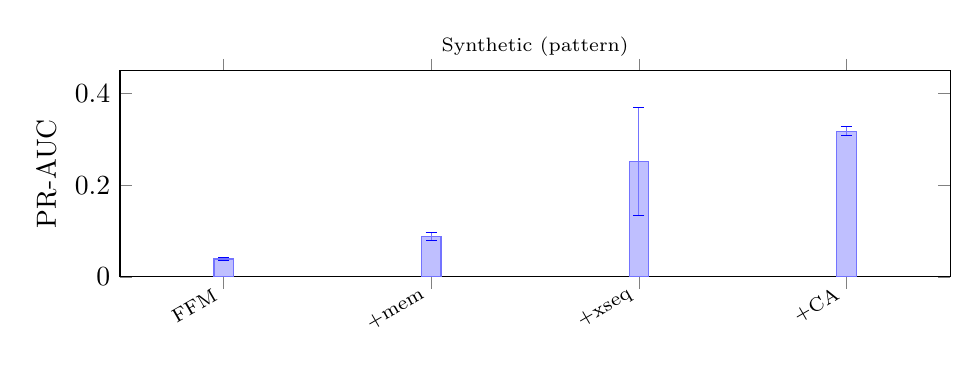
\begin{tikzpicture}
\begin{axis}[width=\linewidth, height=4.2cm, ybar, bar width=7pt,
  ymin=0, ymax=0.45, ylabel={PR-AUC}, ylabel near ticks,
  xmin=0.5, xmax=4.5, xtick={1,2,3,4},
  xticklabels={FFM,+mem,+xseq,+CA}, x tick label style={rotate=30,anchor=east,font=\scriptsize},
  title={\scriptsize Synthetic (pattern)}, title style={yshift=-1ex}]
\addplot+[fill=blue!25, draw=blue!55, error bars/.cd, y dir=both, y explicit] coordinates {
  (1,0.039) +- (0,0.004) (2,0.088) +- (0,0.009)
  (3,0.252) +- (0,0.117) (4,0.318) +- (0,0.010)};
\end{axis}
\end{tikzpicture}
\end{subfigure}\hfill
\begin{subfigure}{0.49\linewidth}\centering
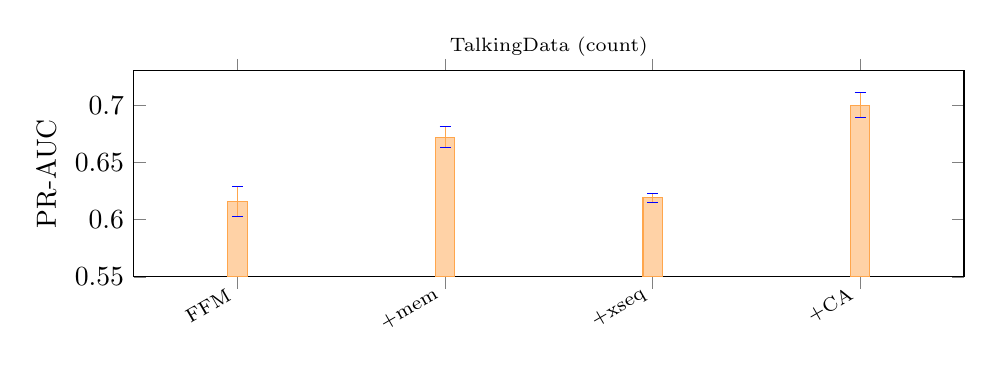
\begin{tikzpicture}
\begin{axis}[width=\linewidth, height=4.2cm, ybar, bar width=7pt,
  ymin=0.55, ymax=0.73, ylabel={PR-AUC}, ylabel near ticks,
  xmin=0.5, xmax=4.5, xtick={1,2,3,4},
  xticklabels={FFM,+mem,+xseq,+CA}, x tick label style={rotate=30,anchor=east,font=\scriptsize},
  title={\scriptsize TalkingData (count)}, title style={yshift=-1ex}]
\addplot+[fill=orange!35, draw=orange!70, error bars/.cd, y dir=both, y explicit] coordinates {
  (1,0.616) +- (0,0.013) (2,0.672) +- (0,0.009)
  (3,0.619) +- (0,0.004) (4,0.700) +- (0,0.011)};
\end{axis}
\end{tikzpicture}
\end{subfigure}
\caption{Count vs.\ pattern, and the unifying fix (PR-AUC, mean\,$\pm$\,std, 3 seeds).
\textbf{Left (synthetic, pattern signal):} raw-neighbour attention (\texttt{+xseq}) has a high mean
but is wildly seed-unstable; the count-aware encoder (\texttt{+CA}) is stable and highest.
\textbf{Right (TalkingData, count signal):} \texttt{+xseq} alone barely moves over the per-account
FFM (a bounded window truncates a velocity magnitude), the memory (count) path helps, and
\texttt{+CA} wins. One module (\texttt{+CA}) is best in both regimes. Note the different $y$-ranges.}
\label{fig:results}
\end{figure}
